\documentclass{beamer}
\mode<presentation>
{
  \usetheme{Madrid}       % or try default, Darmstadt, Warsaw, ...
  \usecolortheme{beaver} % or try albatross, beaver, crane, ...
  \usefonttheme{structurebold}    % or try default, structurebold, ...
  \setbeamertemplate{navigation symbols}{}
  \setbeamertemplate{caption}[numbered]
}

\AtBeginSection[]
{
\setbeamercolor{section in toc}{fg=alerted text.fg}
\setbeamercolor{section in toc shaded}{fg=structure}
\begin{frame}<beamer>
  \frametitle{Table des mati\`eres}
  \tableofcontents[currentsection]
\end{frame}
}

\usepackage[french]{babel}
\usepackage[utf8x]{inputenc}
\usepackage{url}

\usepackage{stackengine}
\usepackage{scalerel}
\usepackage{xcolor}
\newcommand\danger[1][2ex]{%
  \renewcommand\stacktype{L}%
  \scaleto{\stackon[1.3pt]{\color{red}$\triangle$}{\tiny !}}{#1}%
}
\addtobeamertemplate{frame begin}{}{\setlength{\parskip}{1em}}

\title{Atelier musique libre}   
\author{Louvain-li-Nux}
\date{15 mars 2016}

\begin{document}

% What is MAO?
% What will we be learning here?
% Basic knowledge
% Why free software?
% What softwares will we be using?

\frame{\titlepage}

\begin{frame}{Table des matières}
  \tableofcontents
\end{frame}

%%% INTRODUCTION %%%
\section{Introduction}
\subsection{La MAO, qu'est-ce que c'est ?}
\begin{frame}{La MAO, qu'est-ce que c'est ?}
  \textbf{MAO} (musique assistée par ordinateur) = \textit{l'ensemble des utilisations de \textbf{l'informatique} comme outil pour la \textbf{création}, la \textbf{diffusion} et la formation \textbf{musicale}.}
  Cela comprend :
  \begin{itemize}
  \item la composition : séquençage MIDI, boucles musicales, ... ;
  \item l'édition de partitions ;
  \item la lecture de son et la synthèse sonore ;
  \item l'enregistrement audio ;
  \item l'édition audio ;
  \item le traitement du son ;
  \item la conversion et la diffusion ;
  \item et plus encore.
  \end{itemize}
\end{frame}

\begin{frame}{Comment faire de la MAO ?}
  Aspect \textbf{matériel} :
  \begin{itemize}
  \item ordinateur ;
  \item interface audio (carte son) ;
  \item enceintes de monitoring ;
  \item instruments, interfaces MIDI, micros.
  \end{itemize}
  \medskip
  
  Aspect \textbf{logiciel} :
  \begin{itemize}
  \item Windows, Mac ou \textbf{Linux} ;
  \item logiciel d'enregistrement et de montage ;
  \item séquenceur MIDI ;
  \item sampler/échantillonneur et synthétiseur ;
  \item plugins, effets, ...
  \end{itemize}
\end{frame}



\subsection{Contenu et objectifs de ce cours}
\begin{frame}{Contenu de ce cours}
  Ce qu'on \textbf{va} faire :
  \begin{itemize}
  \item apprendre les concepts de base de la MAO ;
  \item apprendre à utiliser certains logiciels libres pour faire de la MAO ;
  \item composer, enregistrer et produire un clip audio.
  \end{itemize}
  \medskip
  
  Ce qu'on \textbf{ne va pas} faire :
  \begin{itemize}
  \item apprendre les bases de la musique ;
  \item apprendre un instrument ;
  \item quoi que ce soit lié à la vidéo.
  \end{itemize}
\end{frame}

\begin{frame}{Objectifs de ce cours}
  Objectif double :
  
  Découvrir la \textbf{MAO} et la puissance des \textbf{logiciels libres}.
  \bigskip
  
  Qu'est-ce que \emph{vous} recherchez dans ce cours ?
\end{frame}



\section{Concepts de base}
\subsection{Le son dans un ordinateur}
\begin{frame}{Le son dans un ordinateur : signal audio}
  \begin{center}
  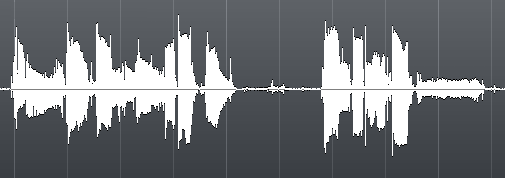
\includegraphics[scale=0.4]{signal_audio.png}
  \end{center}
  
  Un \textbf{signal audio} est la représentation de son dans un ordinateur. Par exemple:
  \begin{itemize}
  \item son de la voix ;
  \item guitare enregistrée ;
  \item musique MP3 ;
  \item de manière générale : tout ce qui sort des enceintes d'un ordinateur.
  \end{itemize}
  On peut modifier un signal audio en y appliquant des effets (écho, reverb, chorus, autotune, \dots).
\end{frame}
\begin{frame}{Le son dans un ordinateur : signal audio}
  \begin{center}
  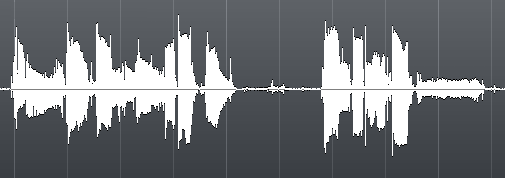
\includegraphics[scale=0.4]{signal_audio.png}
  \end{center}
  
  Différents signaux audio sont combinés en un seul, puis envoyés à la \textbf{carte son} de l'ordinateur. Celle-ci le transforme en un signal continu, qui devient du son dans les enceintes.
\end{frame}

\begin{frame}{Représentation du son : signal MIDI}
  \begin{center}
  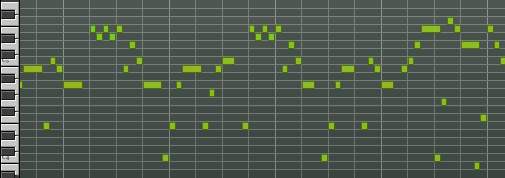
\includegraphics[scale=0.4]{signal_midi.png}
  \end{center}
  
  Un signal MIDI est une représentation des notes d'une musique indépendamment de l'instrument utilisé pour les jouer. Comme une partition, mais compréhensible par un ordinateur.
  \medskip
  
  Un signal MIDI n'est pas écoutable directement. Il doit d'abord être transformé en signal sonore par un logiciel qui va ``jouer la partition''. Deux variantes existent :
  \begin{itemize}
  \item synthétiseur ;
  \item échantillonneur.
  \end{itemize}
\end{frame}

\subsection{Les outils utilisés en MAO}
\begin{frame}{Synthétiseur}
  Un \textbf{synthétiseur} est un appareil ou un programme qui transforme un \emph{signal MIDI} en \emph{signal audio}. Il le fait en \emph{produisant des sons électroniquement}.
  \medskip
  
  Le son produit par un synthétiseur ne ressemble jamais exactement à au son d'un instrument réel, mais ce n'est pas l'objectif. Un synthétiseur est un \emph{instrument à part entière}.
  \medskip
  
  \danger{} Par abus de langage, on désigne souvent le couple clavier + synthétiseur matériel sous le nom ``synthétiseur'', mais le clavier n'est que le contrôleur.
\end{frame}

\begin{frame}{Échantillonneur}
  Un \textbf{échantillonneur} est un programme qui transforme un \emph{signal MIDI} en \emph{signal audio}. Il le fait en jouant des sons réels pré-enregistrés appelés échantillons.
  \medskip
  
  De la même manière qu'une police de caractère possède une image pour chaque lettre, un set d'échantillons possède un ou plusieurs sons pour chaque note.
  \medskip
  
  On utilise un échantillonneur pour reproduire fidèlement le son d'un instrument réel. Plus les échantillons sont de bonne qualité, plus le résultat sera proche de la réalité.
\end{frame}

\begin{frame}{Pistes}
  Un clip audio est composée de plusieurs \textbf{pistes} qui sont soit \textbf{audio} soit \textbf{MIDI}. Une piste est un \textbf{signal enregistré} que l'on peut modifier et mixer.
  \medskip
  
  Faire de la MAO correspond à enregistrer ces pistes, les modifier et les mixer en une seule pour produire le résultat final.
  \medskip
  
  Par exemple, une chanson pourrait avoir une piste par instrument. Individuellement, on décide le niveau sonore de chaque piste, sa position (droite-gauche), les effets, etc. Certaines pistes sont audio (e.g. voix, guitares), d'autres sont MIDI (e.g. clavier, percussions).
\end{frame}

\begin{frame}{Manipuler des pistes}
  On enregistre, édite et mixe des pistes avec des programmes différents en fonction de leur type :
  \begin{itemize}
  \item les pistes audio utilisent un \textbf{éditeur audio} ;
  \item les pistes MIDI utilisent un \textbf{séquenceur}.
  \end{itemize}
  
  En fonction du résultat visé, on va utiliser :
  \begin{itemize}
  \item \textbf{un éditeur audio} pour faire des podcasts, de la musique avec des instruments réels, etc. ;
  \item \textbf{un séquenceur} pour faire de la musique purement électronique ;
  \item \textbf{les deux} pour faire de la musique à la fois électronique et acoustique.
  \end{itemize}
  Beaucoup de logiciels comprennent à la fois un éditeur audio et un séquenceur.
\end{frame}




\section{Les logiciels libres dans la MAO}
\subsection{Brève introduction au libre}
\begin{frame}{Brève introduction au libre}
  %TODO: c'est une parenthèse que je pense utile.
\end{frame}

\subsection{Pourquoi des logiciels libre pour la MAO ?}
\begin{frame}{Pourquoi des logiciels libres pour la MAO ?}
  Il existe beaucoup de solutions propriétaires pour faire de la MAO. On peut citer par exemple Cubase, Pro Tools, FL Studio, Garage Band. Ces logiciels sont très bons et largement utilisés dans le milieu professionnel.
  \medskip
  
  \textbf{Quels sont les intérêts des logiciels libres ?}
  \begin{itemize}
  \item Prix
  \item Qualité
  \item Communauté
  \item Diversité
  \end{itemize}
\end{frame}

\begin{frame}{Pourquoi des logiciels libres pour la MAO ?}
  \begin{itemize}
  \item \textbf{Prix}
  
    Même si libre $\neq$ gratuit, c'est souvent le cas.
    
    Tous les logiciels utilisés dans ce cours sont \textbf{gratuits}, à l'exception de \textbf{Ardour} qui est disponible \textbf{à prix libre}. On recommande néanmoins de faire des dons pour soutenir les projets.
    
  \item \textbf{Qualité}
    
    Malgré leur gratuité, les logiciels libres sont d'excellentes alternatives, en terme de qualité du logiciel, aux concurrents propriétaires.
    
    On peut obtenir des \textbf{résultats pro sans dépenser beaucoup d'argent}. Le rapport qualité-prix est réellement surprenant.
  \end{itemize}
\end{frame}

\begin{frame}{Pourquoi des logiciels libres pour la MAO ?}
  \begin{itemize}
  \item \textbf{Communauté}
  
    L'un des aspects les plus importants du libre. Les logiciels libres sont généralement soutenus par une large communauté ouverte de programmeurs et d'utilisateurs qui contribuent au développement et qui s'entraident.
    
    Communautés de MAO libre :
    \begin{itemize}
    \item francophone : \textbf{\url{linuxmao.org}},
    \item anglophone : \textbf{\url{linuxmusicians.com}}.
    \end{itemize}
    
  \item \textbf{Diversité}
    
    La philosophie du libre pousse à la diversité. Il existe beaucoup de logiciels différents pour faire les même choses. Si ce que vous utilisez ne vous satisfait pas, il est probable qu'une alternative adaptée existe.
  \end{itemize}
\end{frame}

\begin{frame}{En résumé}
  \textbf{Pour les débutants} : aucun engagement, large communauté, logiciels de qualité.
  \medskip
  
  \textbf{Pour les professionnels} : bonne alternative au propriétaire, beaucoup de choix, de plus en plus compétitif.
\end{frame}



\section{Les logiciels que nous allons utiliser}
\begin{frame}{Logiciels que nous allons utiliser}
  Philosophie de la MAO sur Linux : la \textbf{modularité}. Il y a des dizaines de logiciels disponibles pour différents usages, capables d'intéragir entre-eux à travers une même interface : \textbf{Jack}.
  \medskip
  
  Logiciels utilisés dans ce cours :
  \begin{itemize}
  \item Jack et QJackCtl ;
  \item Ardour ;
  \item Hydrogen ;
  \item ZynAddSubFX ;
  \item Qtractor ;
  \item LinuxSampler.
  %TODO: cette liste est à étendre/revisiter
  \end{itemize}
  
  Cela peut sembler beaucoup, mais il faut se rappeler que, généralement, \emph{chaque logiciel fait \textbf{une et une chose}}.
\end{frame}

\subsection{Jack}
\begin{frame}{Jack et QJackCtl}
  \textbf{Jack} est un \textbf{serveur audio}. Il sert à \textbf{connecter} les logiciels entre-eux et avec les interfaces physiques. Tout logiciel de MAO sur Linux possède des interfaces d'entrée et de sortie son et MIDI compatibles avec Jack.
  
  \begin{center}
    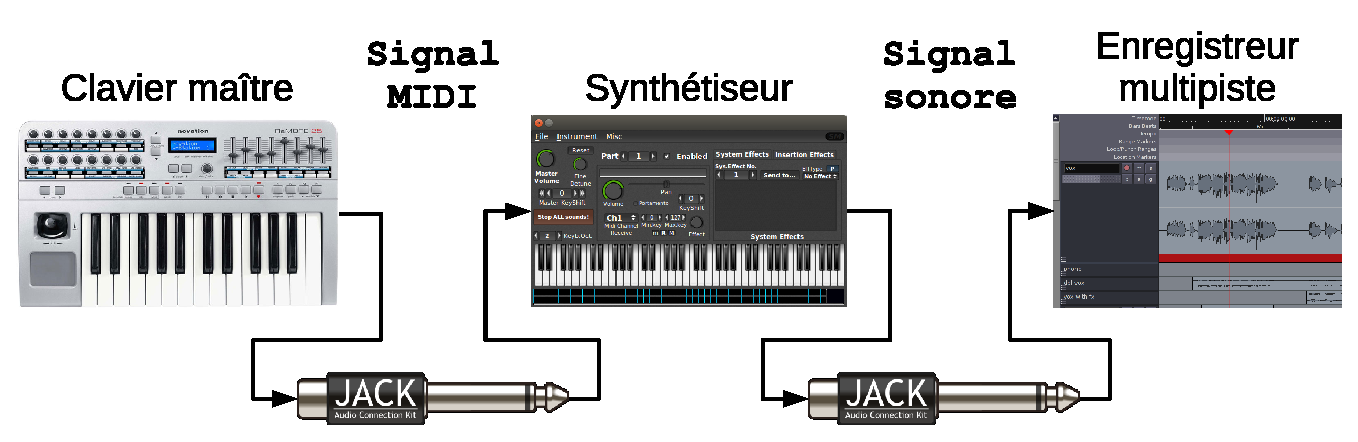
\includegraphics[width=0.8\textwidth]{jack_schema.eps}
  \end{center}
\end{frame}

\begin{frame}{Jack et QJackCtl}
  \textbf{QJackCtl} est une interface graphique pour de Jack. On s'en sert pour manuellement gérer la configuration et les connections de Jack.
  
  \begin{center}
    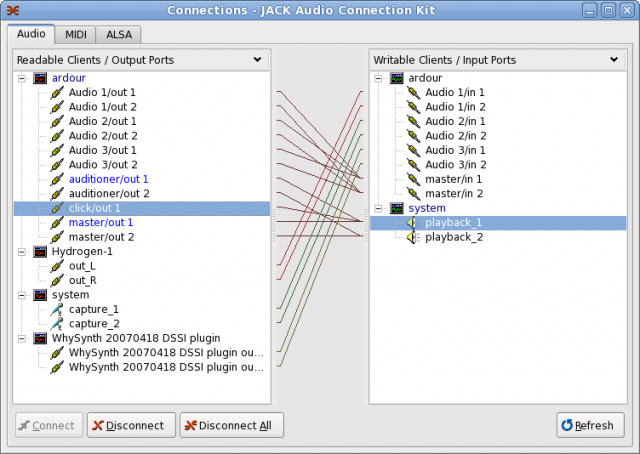
\includegraphics[scale=0.3]{qjackctl_connections.png}
  \end{center}
\end{frame}

\subsection{Ardour}
\begin{frame}{Ardour}
  \begin{columns}
  \begin{column}{0.15\textwidth}
    
\includegraphics[width=\linewidth]{ardour_logo}
  \end{column}
  \begin{column}{0.85\textwidth}
    \textbf{Ardour} est un \textbf{enregistreur multipiste}, ainsi qu'un logiciel de \textbf{montage} et de \textbf{traitement} du son. Il est multi-fonction et comprend à la fois un \textbf{éditeur audio} et un \textbf{séquenceur}. C'est l'outil principal que nous allons utiliser.

    Très complet, de niveau professionnel.
    Il est \textbf{payant}, mais \textbf{le prix est libre}. Vous pouvez l'acheter pour 1\$ ou pour 1M\$.
  \end{column}
  \end{columns}
  \medskip
  
  Avec Ardour, nous allons \textbf{enregistrer} des pistes audio venant :
  \begin{itemize}
  \item du matériel (micros, guitares, etc.) ;
  \item d'autres logiciels (à travers Jack).
  \end{itemize}
  Nous allons \textbf{appliquer des effets} et \textbf{monter} les pistes audio ensemble. Enfin, nous allons \textbf{exporter} le projet en un fichier audio.
\end{frame}

\subsection{Hydrogen}
\begin{frame}{Hydrogen}
  \begin{columns}
  \begin{column}{0.15\textwidth}
    
\includegraphics[width=\linewidth]{hydrogen_logo}
  \end{column}
  \begin{column}{0.85\textwidth}
    \textbf{Hydrogen} est un \textbf{échantillonneur} : un logiciel de synthèse sonore à partir d'échantillons réels. En particulier, Hydrogen est spécialisé dans les \textbf{batteries} et autres \textbf{instruments de percussion}. Il possède également un \textbf{séquenceur} intégré qui permet d'écrire des lignes de batteries.
  \end{column}
  \end{columns}
  \medskip
    
  Avec Hydrogen, nous allons \textbf{simuler des percussions réelles}.
\end{frame}

\subsection{ZynAddSubFX}
\begin{frame}{ZynAddSubFX}
  \begin{columns}
  \begin{column}{0.15\textwidth}
    \def\svgwidth{\linewidth}
    \input{zynaddsubfx_logo.pdf_tex}
  \end{column}
  \begin{column}{0.85\textwidth}
    \textbf{ZynAddSubFX} est un \textbf{synthétiseur} : un logiciel de synthèse sonore, cette fois-ci de manière purement logicielle. Il est très puissant et peut produire une gamme de son très large. Pour les débutants, un grand nombre de presets est disponible.
  \end{column}
  \end{columns}
  \medskip
  
  Avec ZynAddSubFX, nous allons \textbf{simuler des instruments électroniques}.
  Une utilisation avancée étant compliquée, nous allons nous contenter d'utiliser les presets proposés.
\end{frame}

%TODO: LinuxSampler
%TODO: Rosegarden??? Ou alternative

\end{document}

